\begin{figure}[htbp]

\begin{center}
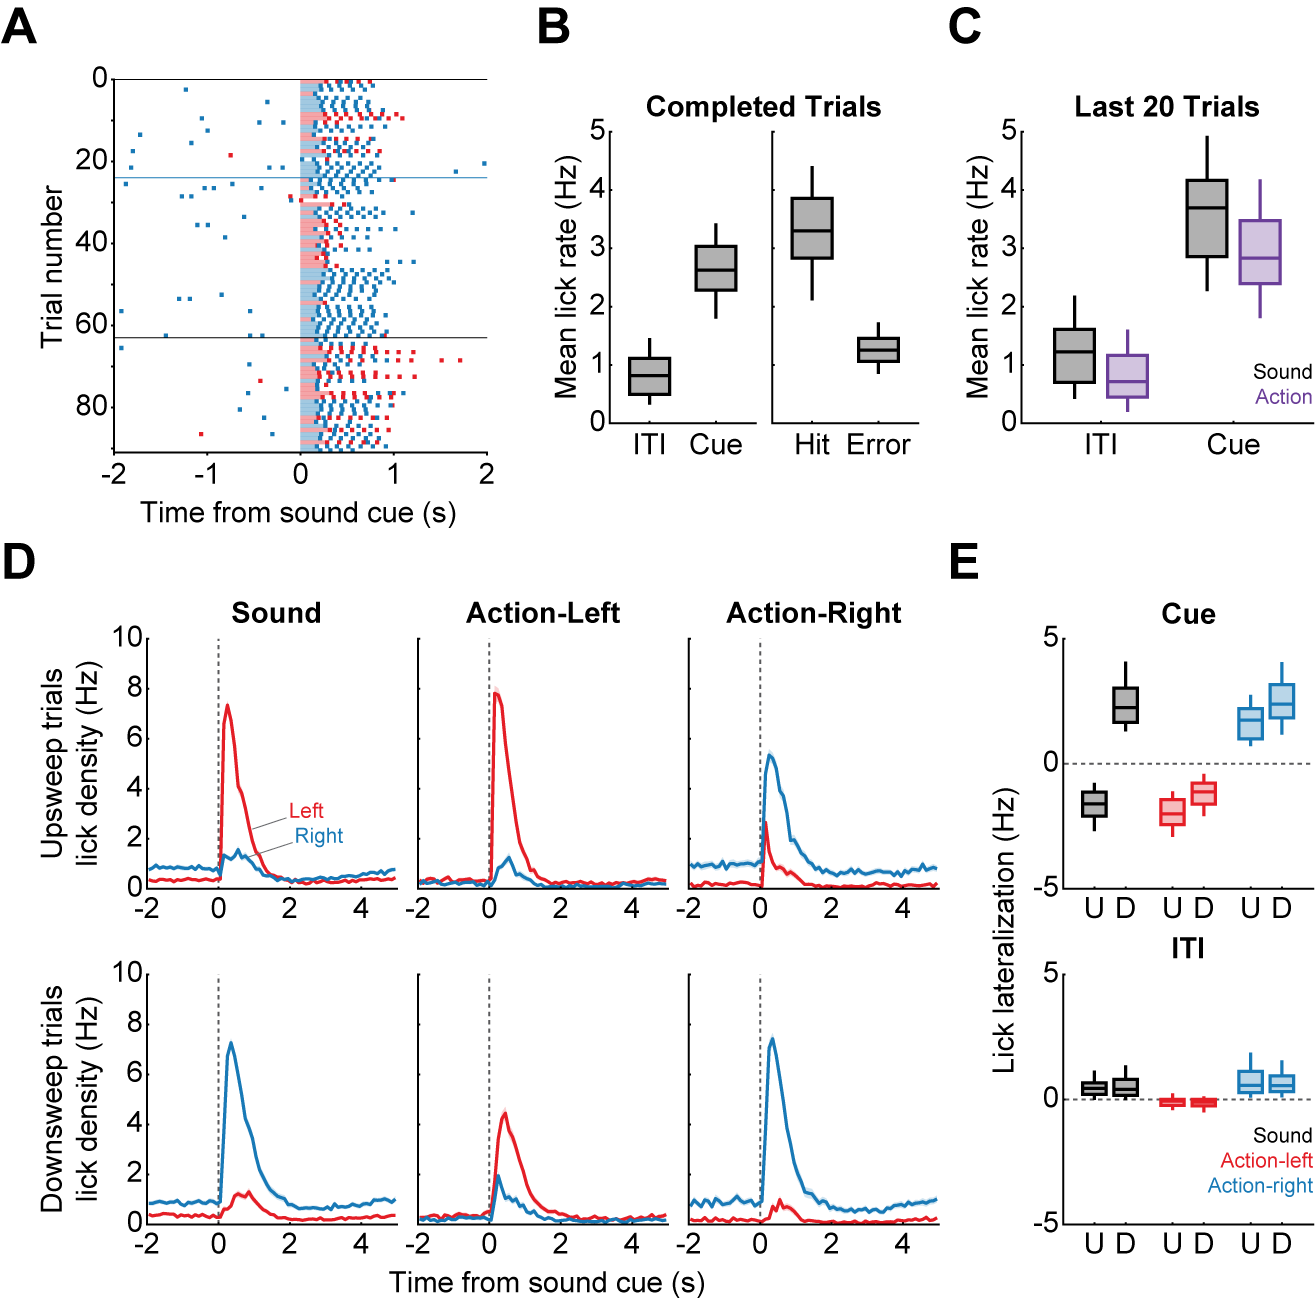
\includegraphics[width=11.4cm]{Figures/Chapter4/Fig2} 
\end{center}

\caption[Dependence of lick output on task structure]
{Dependence of lick output on the task structure. (A) Raster plot of individual lick times, aligned to cue onset during the first three blocks of an example session. Rows of the raster correspond to consecutive trials. The cue period of each trial is highlighted in pale red for upsweeps and pale blue for downsweeps, with red and blue tick marks representing left and right licks, respectively. Fine horizontal lines indicate the first trial of each rule block. The order of the blocks was sound--action-right--sound. (B) Mean lick rates for the 2 s periods before and after cue onset (ITI and Cue, respectively), estimated from all completed trials. Left, overall comparison of ITI and cue periods. Right, comparison of hit and error trials during the cue period. (C) Mean lick rates for the ITI and cue periods, presented separately for sound (black) and action trials (purple). (D) Lick density at the left (red) and right port (blue) across all sessions, calculated in 100 ms time bins surrounding cue onset. Data are plotted separately as the $\mathit{mean} \pm \mathit{SEM}$ for upsweep (top) and downsweep trials (bottom) within each block type. (E) Lick lateralization in upsweep (U) and downsweep trials (D) within each block type. Lick lateralization was calculated as the difference between the number of right and left licks during the 2 s before (bottom) and after cue onset (top) in each trial. Positive and negative values indicate a greater number of right and left licks, respectively. For C--E, analysis was restricted to the last twenty trials of each block: the period in which the accuracy criterion was met. For B--E, $N = 64$ sessions. Box plots in all figures represent quartiles 1--3 for each group. Whiskers indicate the 9th and 91st percentiles.}

\label{fig:Fig2}
\end{figure}
